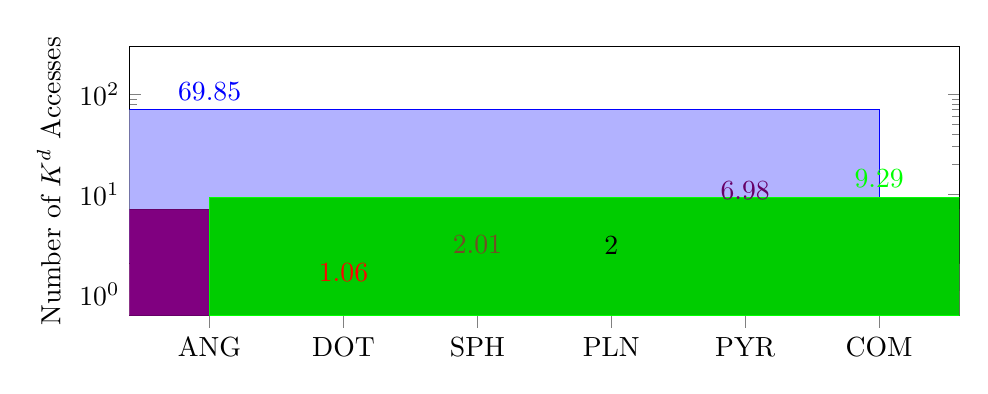
\begin{tikzpicture}
    \begin{axis}[
    ybar,
    width=\linewidth, height=5cm,
    ylabel={Number of $K^d$ Accesses}, ylabel near ticks, ymin=0, ymax=300,
    xticklabels={ANG, DOT, SPH, PLN, PYR, COM},
    xtick={1, 2, 3, 4, 5, 6}, xmin=0.4, xmax=6.6, xtick pos=left, point meta=rawy,
    nodes near coords, nodes near coords align={vertical},
    ymode=log, log origin=infty,
    every axis plot/.append style={
    ybar,
    bar width=10,
    bar shift=0pt,
    fill
    }
    ]
        \addplot coordinates {(1, 69.85)};
        \addplot coordinates {(2, 1.06)};
        \addplot coordinates {(3, 2.01)};
        \addplot coordinates {(4, 2.00)};
        \addplot coordinates {(5, 6.98)};
        \addplot coordinates {(6, 9.29)};
    \end{axis}
\end{tikzpicture}

%SELECT AVG(PercentageCorrect), IdentificationMethod, AVG(QueryCount)
%FROM IDENTIFICATION
%WHERE ShiftDeviation < 1.0e-7 AND FalseStars = 0
%GROUP BY IdentificationMethod